%%%%%%%%%%%%%%%%%%%%%%%%%%%%%%%%%%%%%%%%%
% a0poster Portrait Poster
% LaTeX Template
% Version 1.0 (22/06/13)
%
% The a0poster class was created by:
% Gerlinde Kettl and Matthias Weiser (tex@kettl.de)
%
% This template has been downloaded from:
% http://www.LaTeXTemplates.com
%
% License:
% CC BY-NC-SA 3.0 (http://creativecommons.org/licenses/by-nc-sa/3.0/)
%
%%%%%%%%%%%%%%%%%%%%%%%%%%%%%%%%%%%%%%%%%

%----------------------------------------------------------------------------------------
%	PACKAGES AND OTHER DOCUMENT CONFIGURATIONS
%----------------------------------------------------------------------------------------

\documentclass[a0,portrait]{a0poster}

\usepackage{multicol} % This is so we can have multiple columns of text side-by-side
\columnsep=100pt % This is the amount of white space between the columns in the poster
\columnseprule=3pt % This is the thickness of the black line between the columns in the poster

\usepackage[svgnames]{xcolor} % Specify colors by their 'svgnames', for a full list of all colors available see here: http://www.latextemplates.com/svgnames-colors

\usepackage{times} % Use the times font
%\usepackage{palatino} % Uncomment to use the Palatino font

\usepackage{graphicx} % Required for including images
\graphicspath{{figures/}} % Location of the graphics files
\usepackage{booktabs} % Top and bottom rules for table
\usepackage[font=small,labelfont=bf]{caption} % Required for specifying captions to tables and figures
\usepackage{amsfonts, amsmath, amsthm, amssymb} % For math fonts, symbols and environments
\usepackage{wrapfig} % Allows wrapping text around tables and figures

\usepackage{color}
\definecolor{dark_blue}{rgb}{0.0,0.0,0.7}
\definecolor{fielddrab}{rgb}{0.42, 0.33, 0.12}

\usepackage{textcomp}
\usepackage{listings}
\lstset{upquote=true,basicstyle=\footnotesize}
\lstdefinelanguage{cml}
{
  identifierstyle=\color{dark_blue},
  morestring=[b]",
  stringstyle=\color{fielddrab},
  morecomment=[l]{--},
  commentstyle = \color{black},
  morekeywords={,@abstraction,@concept,@task,@association,
  and,or,xor,implies,unless,xor?,or?,is,isnt,as,as?,as!,if,then,else,for,in,}
}

\usepackage{verbatim}
\makeatletter
\newcommand{\verbatimfont}[1]{\renewcommand{\verbatim@font}{\ttfamily#1}}
\makeatother

\begin{document}

%----------------------------------------------------------------------------------------
%	POSTER HEADER
%----------------------------------------------------------------------------------------

% The header is divided into two boxes:
% The first is 75% wide and houses the title, subtitle, names, university/organization and contact information
% The second is 25% wide and houses a logo for your university/organization or a photo of you
% The widths of these boxes can be easily edited to accommodate your content as you see fit

\begin{minipage}[b]{0.75\linewidth}
\veryHuge \color{NavyBlue} \textbf{Reusing Conceptual Models} \color{Black}\\[0.5cm] % Title
\Huge\textit{A Conceptual Modeling Language and Extensible Compiler}\\[2.0cm] % Subtitle
\huge \textbf{Quenio Cesar Machado dos Santos \& Raul Sidnei Wazlawick}\\[0.5cm] % Author(s)
\huge Computer Sciences, Universidade Federal de Santa Catarina, Brazil\\[0.4cm] % University/organization
\Large \texttt{quenio.santos@grad.ufsc.br \& raul@inf.ufsc.br} \\
\end{minipage}
%
\begin{minipage}[b]{0.25\linewidth}
\includegraphics[width=12cm]{logo.eps}\\
\end{minipage}

\vspace{1cm} % A bit of extra whitespace between the header and poster content

%----------------------------------------------------------------------------------------

\begin{multicols}{3} % This is how many columns your poster will be broken into, a portrait poster is generally split into 2 columns

%----------------------------------------------------------------------------------------
%	ABSTRACT
%----------------------------------------------------------------------------------------

\color{Navy} % Navy color for the abstract

\begin{abstract}

Presents a textual programming language for conceptual modeling
(based on UML classes/associations and OCL constraints)
and its compiler that can generate code in any target language or technology
via extensible textual templates,
both currently under initial stage of development.
The language and compiler should allow the specification of information
managed by ever-changing, increasingly distributed software systems.
From a single source,
automated code generation should keep implementations consistent with the specification
across the different platforms and technologies.
As the technology landscape evolves,
the target templates may be extended to embrace new technologies.
Unlike other approaches,
such as MDA and MPS,
the textual nature of this modeling language and its extensible templates
is expected to facilitate the integration of model-driven software development
into the workflow of software developers.

\end{abstract}


%----------------------------------------------------------------------------------------
%	INTRODUCTION
%----------------------------------------------------------------------------------------

\color{SaddleBrown} % SaddleBrown color for the introduction

\section*{Introduction}

This conceptual modeling language and its extensible compiler
are an alternative to the Metaprogramming System (MPS),
as presented by Voelter \cite{voelter}.
While MPS is an integrated development environment
based on domain-specific languages (DSLs),
this proposal (henceforth called CML) is a compiler that:

\begin{itemize}

\item accepts as \emph{input} source files coded
in its own conceptual modeling language,
which has an abstract syntax similar to
(but less comprehensive than)
a combination of UML \cite{uml} and OCL \cite{ocl}.

\item generates as \emph{output} target files in any programming language,
which is accomplished by text-based extensible templates,
provided by the base library bundled with the compiler,
by third-parties, or still by the developers themselves.

\end{itemize}

Figure \ref{fig:architecture} shows an overview of
the CML compiler's arquitecture.

\begin{center}
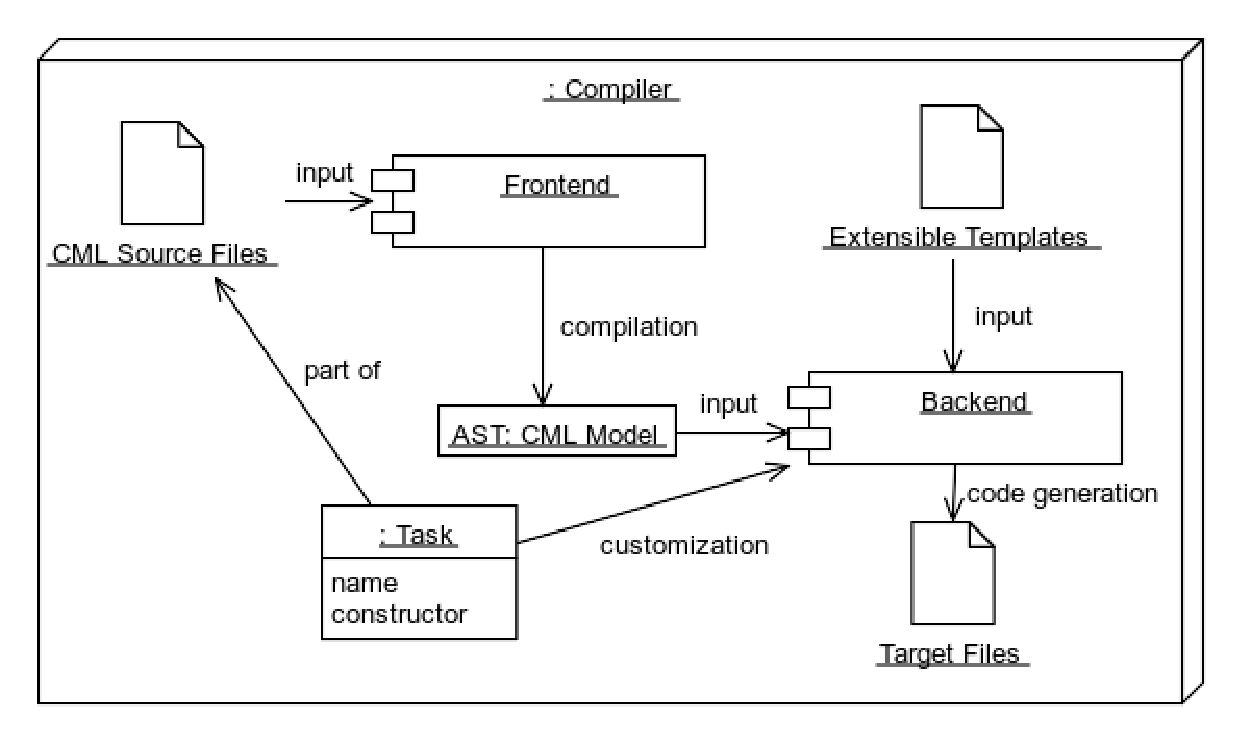
\includegraphics[width=1.0\linewidth]{figures/architecture.eps}
\captionof{figure}{\color{Green} Architectural Overview of CML Compiler}
\label{fig:architecture}
\end{center}

%----------------------------------------------------------------------------------------
%	OBJECTIVES
%----------------------------------------------------------------------------------------

\color{DarkSlateGray} % DarkSlateGray color for the rest of the content

\section*{Main Objectives}

\begin{enumerate}

\item Following the principle established by
the \emph{Conceptual-Model Programming (CMP) manifesto} \cite{cmp},
CML intends to enable modeling-as-programming,
allowing software developers to incorporate conceptual modeling
into the same workflow they are used to doing software development.

\item In order to validate the use of the CML language and compiler
to model and implement its own metamodel,
this initial version of CML provides
generalization/specialization,
associations with cardinality zero-or-one (optionals)
and zero-or-more (sequences),
and the ability to define derived atributes/associations
using expressions.

\item CML allows developers to customize and extend
the generated code via extensible templates
in order to leverage conceptual models
across different programming languages and technologies.

\item While other initiatives,
such as the \emph{Model-Driven Architecture} \cite{mda},
require the use of languages and tools from different vendors,
CML combines into a single, open-source language/compiler package,
the ability to model and to customize code generation,
allowing models to last a longer lifespan
than it is normally viable with specific technologies.

\end{enumerate}

%----------------------------------------------------------------------------------------
%	MATERIALS AND METHODS
%----------------------------------------------------------------------------------------

\section*{The Language}

\subsection*{Generalization/Specialization}

Figure \ref{ex:generalization} presents some examples of
generalization/specialization relationships defined in CML.

\begin{center}
\verbatimfont{\small}
\lstinputlisting[language=cml]{examples/generalization.cml}
\captionof{figure}{\color{Green} Generalization/Specialization in CML}
\label{ex:generalization}
\end{center}

\subsection*{Associations}

Figure \ref{ex:associations} presents some examples of \emph{associations} defined in CML.

\begin{center}
\verbatimfont{\small}
\lstinputlisting[language=cml]{examples/associations.cml}
\captionof{figure}{\color{Green} Associations in CML}
\label{ex:associations}
\end{center}

%----------------------------------------------------------------------------------------
%	RESULTS
%----------------------------------------------------------------------------------------

\section*{Extensible Templates}

Figure \ref{ex:associations} presents some examples of
\emph{extensible templates} defined in StringTemplate \cite{st}.

\begin{center}
\verbatimfont{\scriptsize}
\begin{minipage}{\linewidth}
\lstinputlisting{examples/example.stg}
\end{minipage}
\captionof{figure}{\color{Green} Extensible Templates}
\label{ex:templates1}
\end{center}

%----------------------------------------------------------------------------------------
%	CONCLUSIONS
%----------------------------------------------------------------------------------------

\color{SaddleBrown} % SaddleBrown color for the conclusions to make them stand out

\section*{Related Work}

When compared to CML, the text-based languages are the most relevant.
MPS \cite{voelter} is a development environment for DSLs.
Strictly speaking, its DSLs are not textual,
since their AST is directly edited on projectional editors.
However, the editors allow textual representations.
Unlike MPS,
the DSLs created with the M language \cite{mlang} are truly textual.
It was part of the discontinued Oslo project from Microsoft,
which incorporated into Visual Studio similar capabilities to what is available on MPS.
Xtext/Xtend \cite{xtext} allows the definition of textual DSLs
to generate code from conceptual models edited on Eclipse.
It is similar to the Oslo project from Microsoft,
and based on EMF \cite{emf}.
MM-DSL \cite{mm-dsl}, on the other hand,
allows the definition of metamodels (abstract syntax; not the actual DSLs),
which serve as input to generate domain-specific modeling tools.
ThingML \cite{thingml} is also a language and code generation framework for
the development of software in embedded devices.

\color{DarkSlateGray} % Set the color back to DarkSlateGray for the rest of the content

 %----------------------------------------------------------------------------------------
%	REFERENCES
%----------------------------------------------------------------------------------------

\nocite{*} % Print all references regardless of whether they were cited in the poster or not
\bibliographystyle{plain} % Plain referencing style
\bibliography{sample} % Use the example bibliography file sample.bib

%----------------------------------------------------------------------------------------

\end{multicols}
\end{document}
